\documentclass[aspectratio=169]{beamer}
\usepackage{will_handley}

% Commands
% --------
% - \arxiv{arxiv number}
% - \cols{width}{lh column}{rh column}
% -  \begin{fig(left|right)}[fractional width (e.g 0.6) ]{name of image}
%        content of other column
%    \end{fig(left|right)}

% Talk details
% ------------
\title{Nested sampling}
\subtitle{An efficient and robust Bayesian inference tool for 21cm cosmology}
\date{21\textsuperscript{st} October 2020}

% Abstract
% --------
% Nested sampling: an efficient and robust Bayesian inference tool for 21cm
% cosmology
% 
% Nested sampling is an alternative Markov-chain Monte-Carlo technique for
% integrating and exploring probability distributions. With publicly available
% implementations such as MultiNest, PolyChord and dynesty, nested sampling has
% become widely adopted in astronomy as a powerful tool for computing Bayesian
% evidences and sampling challenging a-priori unknown parameter spaces.
% 
% In this talk I will give a user's guide to the theory of nested sampling in
% the context of 21cm Bayesian model comparison and parameter estimation, a
% survey of the current state of the art and the future of the field. This will
% aim to provide theoretical background for the Bayesian inference techniques
% and algorithms underpinning the science of several other talks which focus on
% applying nested sampling to 21cm cosmology.

\begin{document}

\begin{frame}
    \titlepage
\end{frame}

\begin{frame}
    \frametitle{Bayesian inference in global 21cm cosmology}
    \begin{itemize}
        \item Data analysis problem
            \begin{align}
                \text{Data} &= \text{Signal} + \text{Foreground} + \text{Noise} \nonumber\\
                T_\text{data}(\nu) &= T_\text{21cm}(\nu;\theta_\text{21cm}) + T_\text{fg}(\nu;\theta_\text{fg}) + T_\text{noise}(\nu)
                \nonumber
            \end{align}
        \item We  can only statistically describe $T_\text{noise}$ 
            \begin{itemize}
                \item e.g. as an (un)correlated Gaussian random variable $P(T_\text{noise}) = \frac{1}{\sqrt{2\pi}\sigma} e^{-T_\text{noise}^2/2\sigma^2}$
            \end{itemize}
        \item Allows us to form a {\em likelihood} for the unknown parameters $\theta = (\theta_\text{21cm},\theta_\text{fg})$
            \begin{align}
                \mathcal{L}(\theta) &= P(\text{Data}|\theta) \propto e^{-\frac{1}{2}\chi(\theta)^2} \nonumber\\
                \chi^2(\theta) &= \sum_\nu\frac{1}{\sigma_\nu^2}{\left[T_\text{data}(\nu)-T_\text{21cm}(\nu;\theta_\text{21cm}) - T_\text{fg}(\nu;\theta_\text{fg})\right]}^2
                \nonumber
            \end{align}
        \item This misses the initial step of data compression (reduction, flagging, integration)
        \item In practice also include $\theta_\text{noise}$ as parameters as well.
    \end{itemize}
\end{frame}

\begin{frame}
    \frametitle{The three pillars of Bayesian inference}
    \begin{itemize}
        \item Frequentist approaches maximise the likelihood $\mathcal{L}(\theta) = P(D|\theta)$
            \begin{itemize}
                \item anything using a ``least squares'' optimisation (e.g. \texttt{maxsmooth}, EDGES calibration)
            \end{itemize}
        \item Bayes theorem allows us to answer science questions using probabilities:
    \end{itemize}
    \begin{description}
        \item[Parameter estimation] Given a model, which range of parameters best describe the data?
            \[
                P(\theta|D,M) = \frac{P(\theta|D,M) P(\theta|M)}{P(D|M)}, \qquad
                \text{Posterior} = \frac{\text{Likelihood} \times \text{Prior}}{\text{Evidence}}
            \]
        \item[Model comparison] Which models do the data prefer?
            \[
                P(M|D) = \frac{P(D|M) P(M)}{P(D)}, \qquad
                \text{Model Probability} = \frac{\text{Evidence} \times \text{Model Prior}}{\text{Normalisation}}
            \]
        \item[Tension quantification] Are different (sub)sets of data consistent with one another? %\arxiv{1902.04029}\arxiv{1903.06682}
    \end{description}
\end{frame}

\begin{frame}
    \frametitle{Model comparison in 21cm cosmology}
    \begin{itemize}
        \item Model comparison: Given this data, what odds would a bookmaker put on a model?
        \item In general in 21cm cosmology model takes the form $T_\text{data} = T_\text{21cm} + T_\text{fg} + T_\text{noise}$ 
        \item Model comparison can be applied to any combination of these pieces
    \end{itemize}
    \begin{enumerate}
        \item Does the data contain a signal? \\(Does $T_\text{data} = T_\text{21cm} + T_\text{fg} + T_\text{noise}$ have a higher evidence than $T_\text{data} = T_\text{fg} + T_\text{noise}$)
        \item Which foreground model is better? (polynomial vs forward sky model)
        \item Which noise model is better? (correlated gaussian, uncorrelated gaussian, lorentzian)
        \item How many components should a foreground model have?
        \item How many components should a calibration model have?
    \end{enumerate}
\end{frame}


\begin{frame}
    \frametitle{Numerical tools}
    \cols{
        \begin{itemize}
            \item The key concept in numerical Bayesian inference is \emph{sampling} a distribution 
            \item i.e. drawing parameter vectors $\theta$ in proportion to the probability density $P(\theta)$.
            \item Compression of high-dimensional function.
            \item Posterior $P(\theta|D)$ encodes multidimensional generalisation of error bars
            \item Sampling is traditionally accomplished using random-walk MCMC tools like Gibbs sampling, Metropolis-Hastings, emcee or Hamiltonian Monte Carlo.
        \end{itemize}
    }{
        \includegraphics<1>[width=\textwidth]{params.pdf}
        \includegraphics<2|handout:0>[width=\textwidth]{reach.pdf}
        \includegraphics<3|handout:0>[width=\textwidth]{params_full.pdf}
    }
    
\end{frame}

\begin{frame}
    \frametitle{Nested sampling in action}
    \cols[0.6]{
  \begin{itemize}
    \item Nested sampling is a completely different way of sampling. 
    \item Uses ensemble sampling to compress prior to posterior.
      \item Maintain a set $S$ of $n$ samples, which are sequentially updated:
  \begin{description}
      
    \item[$S_0$:] Generate $n$ samples uniformly over the space (from the prior $\pi$). 
      
    \item[$S_{n+1}$:] Delete the lowest likelihood sample in $S_{n}$, and replace it with a new uniform sample with higher likelihood
  \end{description}
 \item Requires one to be able to uniformly within a region, subject to a {\em hard likelihood constraint}.
  \end{itemize}
    }{
        \includegraphics<1|handout:0>[width=\textwidth,page=1]{himmelblau}
        \includegraphics<2|handout:0>[width=\textwidth,page=2]{himmelblau}
        \includegraphics<3|handout:0>[width=\textwidth,page=3]{himmelblau}
        \includegraphics<4          >[width=\textwidth,page=4]{himmelblau}
        \includegraphics<5|handout:0>[width=\textwidth,page=5]{himmelblau}
        \includegraphics<6|handout:0>[width=\textwidth,page=6]{himmelblau}
        \includegraphics<7|handout:0>[width=\textwidth,page=7]{himmelblau}
        \includegraphics<8|handout:0>[width=\textwidth,page=8]{himmelblau}
        \includegraphics<9|handout:0>[width=\textwidth,page=14]{himmelblau}
    }
\end{frame}


\begin{frame}
    \frametitle{Nested sampling in action}
    \cols[0.6]{
  \begin{itemize}
      \item At the end, one is left with a set of discarded points
      \item These may be weighted to form posterior samples
      \item They can also be used to calculate the evidence
      \item The evolving ensemble of live points allows algorithms to perform self-tuning and mode clustering
  \end{itemize}

    }{
        \includegraphics<1|handout:0>[width=\textwidth,page=14]{himmelblau}
        \includegraphics<2          >[width=\textwidth,page=15]{himmelblau}
    }

\end{frame}

\begin{frame}
    \frametitle{Implementations of Nested Sampling}
    %\begin{columns}
    %    \begin{column}{0.33}
    %        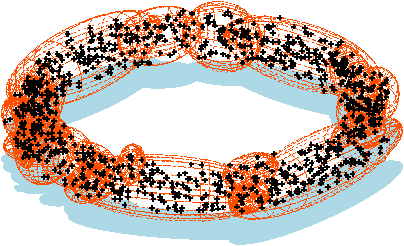
\includegraphics[width=\textwidth]{multinest}
    %    \end{column} 
    %\end{columns}
    \cols[0.5]{%
        \texttt{MultiNest}
        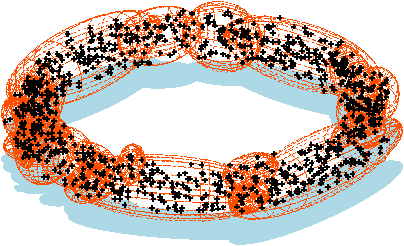
\includegraphics[width=0.8\textwidth]{multinest}
            \vfill
        \texttt{DNest}
        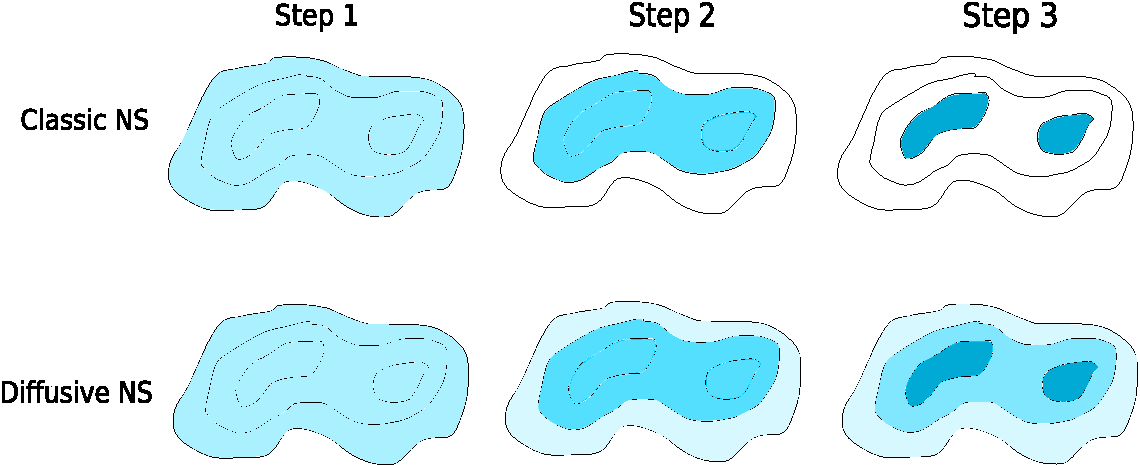
\includegraphics[width=\textwidth]{dnest}
    }{%
        \texttt{PolyChord}
        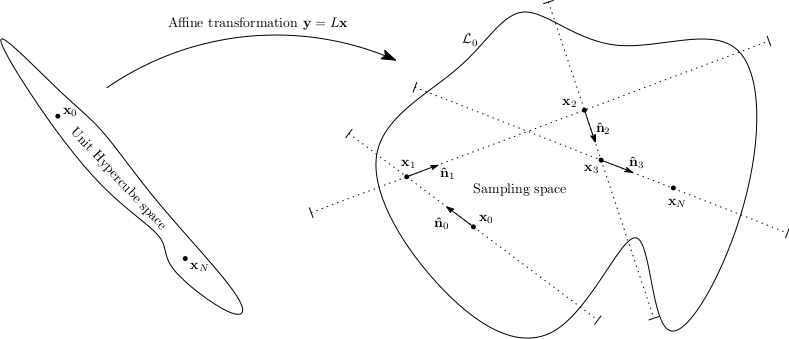
\includegraphics[width=\textwidth]{polychord}
        \vfill
        \texttt{NeuralNest}
            \cols[0.5]{
                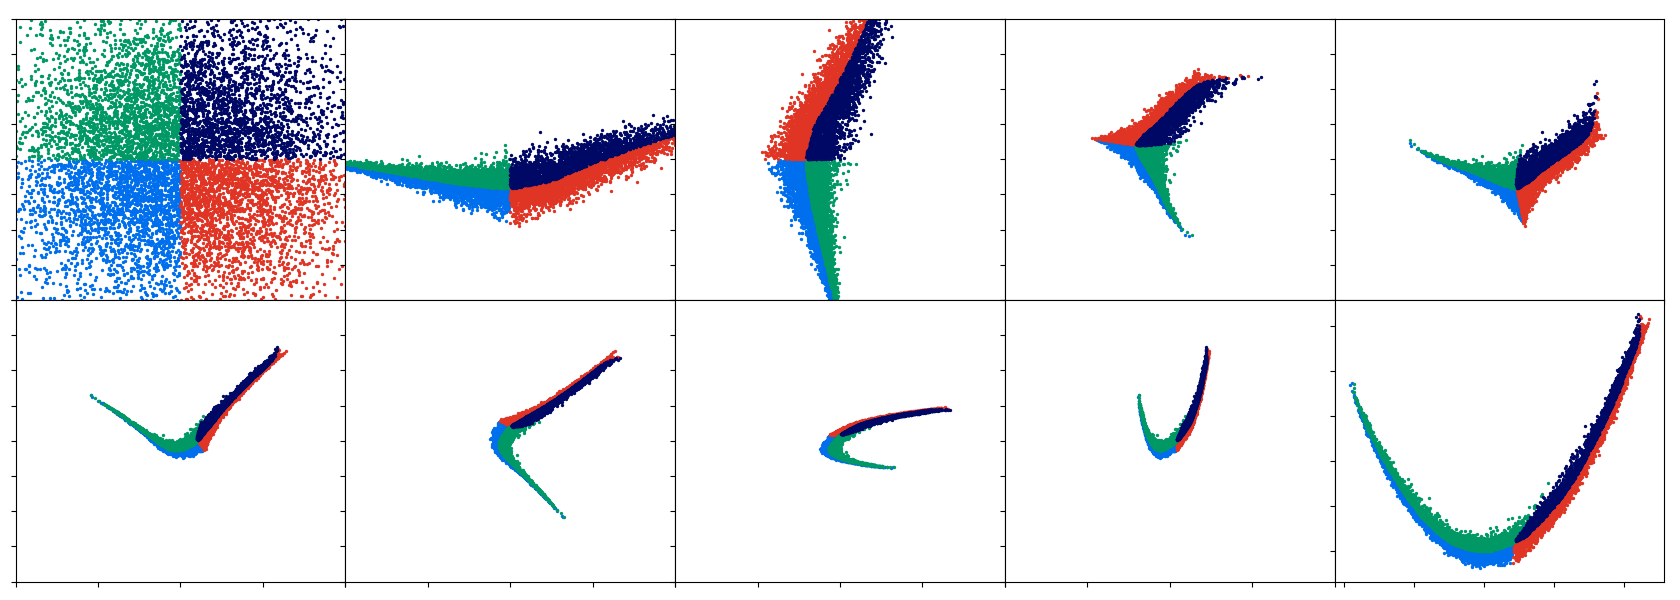
\includegraphics[width=\textwidth]{rosenbrock_flow.png}
                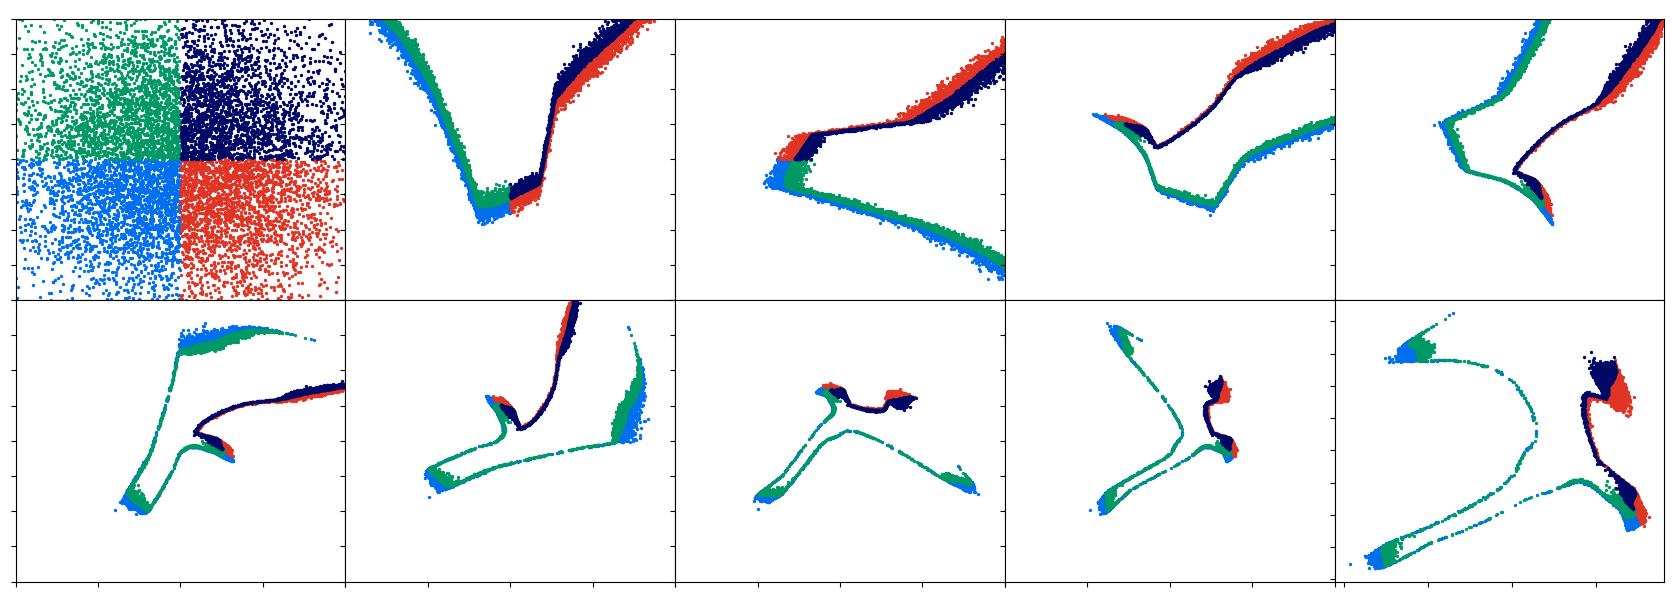
\includegraphics[width=\textwidth]{himmelblau_flow.png}
            }{
                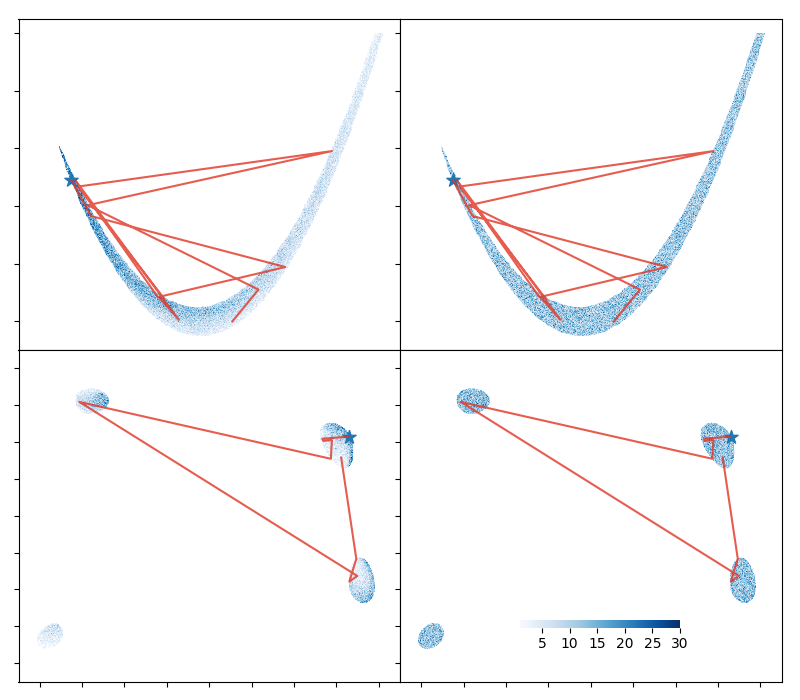
\includegraphics[width=\textwidth]{chains.png}
            }
            \vfill
    }
\end{frame}

\begin{frame}
    \frametitle{Nested Sampling: Benefits and drawbacks}
    Relative to traditional numerical posterior samples (Metropolis Hastings, HMC, emcee), nested sampling:
    \begin{description}
        \item[$+$] Can calculate evidence (and therefore perform model comparison).
        \item[$+$] Can handle multi-modal distributions.
        \item[$+$] Requires little tuning for an a-priori unseen problem.
        \item[$+$] Highly parallelisable ($n_\mathrm{cores} \sim n_\mathrm{live} \gg 4$).
        \item[$-$] Slower than a well-tuned posterior sampler.
        \item[$-$] Run time is dependent on prior choice, and priors must be proper \\(some people view this as a feature rather than a bug).
    \end{description}
\end{frame}


\begin{frame}
    \frametitle{Nested Sampling: a user's guide}
    \begin{enumerate}
        \item Nested sampling is a likelihood scanner, rather than posterior explorer.
            \begin{itemize}
                \item This means typically most of its time is spent on burn-in rather than posterior sampling
                \item Changing the stopping criterion from $10^{-3}$ to $0.5$ does little to speed up the run, but can make results very unreliable
            \end{itemize}
        \item The number of live points $n_\mathrm{live}$ is a resolution parameter.
            \begin{itemize}
                \item Run time is linear in $n_\mathrm{live}$, posterior and evidence accuracy goes as $\frac{1}{\sqrt{n_\mathrm{live}}}$.
                \item Set low for exploratory runs $\sim\mathcal{O}(10)$ and increased to $\sim\mathcal{O}(1000)$ for production standard.
            \end{itemize}
        \item Most algorithms come with additional reliability parameter(s).
            \begin{itemize}
                \item e.g. \texttt{MultiNest}: $\text{eff}$, \texttt{PolyChord}: $n_\mathrm{repeats}$
                \item These are parameters which have no gain if set too conservatively, but increase the reliability
                \item Check that results do not degrade if you reduce them from defaults, otherwise increase.
            \end{itemize}
    \end{enumerate}
\end{frame}


\begin{frame}
    \frametitle{Key tools}
    \begin{description}
        \item[\texttt{anesthetic}] Nested sampling post processing \arxiv{1905.04768}\\
        \item[\texttt{insertion}] cross-checks using order statistics \arxiv{2006.03371}
            \hspace{5pt}\url{github.com/williamjameshandley/anesthetic}
        \item[\texttt{nestcheck}] cross-checks using unthreaded runs \arxiv{1804.06406}\\
            \hspace{5pt}\url{github.com/ejhigson/nestcheck}
        \item[\texttt{MultiNest}] Ellipsoidal rejection sampling \arxiv{0809.3437}\\
            \hspace{5pt}\url{github.com/farhanferoz/MultiNest}
        \item[\texttt{PolyChord}] Python/C++/Fortran state of the art \arxiv{1506.00171}\\
            \hspace{5pt}\url{github.com/PolyChord/PolyChordLite} 
        \item[\texttt{dynesty}] Python re-implementation of several codes \arxiv{1904.02180}\\
            \hspace{5pt}\url{github.com/joshspeagle/dynesty}
    \end{description}
\end{frame}

\end{document}
